\documentclass[10pt]{article}
\usepackage{graphicx}

\title{Demographic Inclusiveness in Human Cell Studies}

\begin{document}
\maketitle
  
\section{Introduction}
  
The research process for preclinical studies typically progresses from cell models, to animal models, and finally human models. During the cell model stage, donors provide a sample of cells to be grown in a lab environment. The possibility of demographic bias in cell culture studies specifically the gender, age and ethnicity of human donors supplying to the cells used for research can have significant consequences for the validity of findings during early stage pharmaceutical studies. However, federal regulations require broad spectrum representation of gender, age and ethnicity during only the final phase of clinical testing, the human model stage. What happens in the first phase of cell models is not regulated and consequently can result in demographic bias. Research question that this study will address is what criteria biologists use when selecting cell sources for early studies and the research objective is to investigate whether there a quantifiable bias in extant literature for cell model studies.

The human genome's major structures recur across the global population regardless of geographical ancestry, self-identified race or sociocultural considerations \cite{xie2001molecular, cooper2003race}. Still, comparatively minor genetic variants generate predictable alterations in the therapeutic impact of some pharmaceutical treatments. Clustering patients by genotype informs the course of drug therapies during treatment of cancer and organ transplant \cite{krynetski2000genetic, higashi2002association}. Because of all of that, the US Food and Drug Administration (FDA) recognized genetic factors sensitize pharmaceutical efficacy and responded by implementing the Demographic Rule in 1998. The rule standardizes race and ethnicity representative during clinical trails based on the target therapeutic population as identified by the drug's sponsor. 

A study published in Science showed that racial and ethnicity diversity serves as an unsubstantiated proxy for broad spectrum representation of genetic variants during clinical trials \cite{haga2003fda}. A retrospective of the FDA's review of clinical trail protocols identified 10\% of the 185 products approved from 1995-1999 disclosed racial differences in the performance of the product on the label \cite{evelyn2001participation}. Moreover, the same study showed that the clinical trials from 1995 - 1999 disclosed the race of participants for 53\% of the nearly 500 k individuals enrolled in  them. Of the 260 k participants whose race was specified, white was most common (88\%), African American was comparable to US population percentage (8\%), and the report classified Hispanics as underrepresented with 1\% of participants.

Demographic bias in clinical trials is an important issue and has already been featured in top notch journals as Science and Nature. However, demographic bias in cell models has not been yet investigated and poses an interesting research question that should be pursued in more details. Not only could results of this study be published in previously mentioned prestigious journals, but this study could also have a broader impact to enhance knowledge of inefficiencies within the drug discovery process and perhaps to raise questions which could lead to extend FDA's Demographic Rule to cell models phase as well. The proposed work aligns with current efforts to vet the efficacy and toxicity of drug candidates early in the discovery process and the intellectual merit of the proposed research lies in expanding the decision criteria for cell sources during the discovery process for an abridged implementation of personalized medicine. 


\section{Data set}

Our data set consist of 36,056 full text papers that are downloaded from Medline and Scopus databases and were tagged as papers working with \textit{stem cells}. Every paper in our data set comes with the full text, but also consist of metadata. Using this data we can explore distribution of papers per years (see Figure \ref{dist1}). More than 95 \% of papers in our data set are published after 2000. We can also see that the data set we are using does not contain all papers for 2014. 

\begin{figure}[b!]
\centering
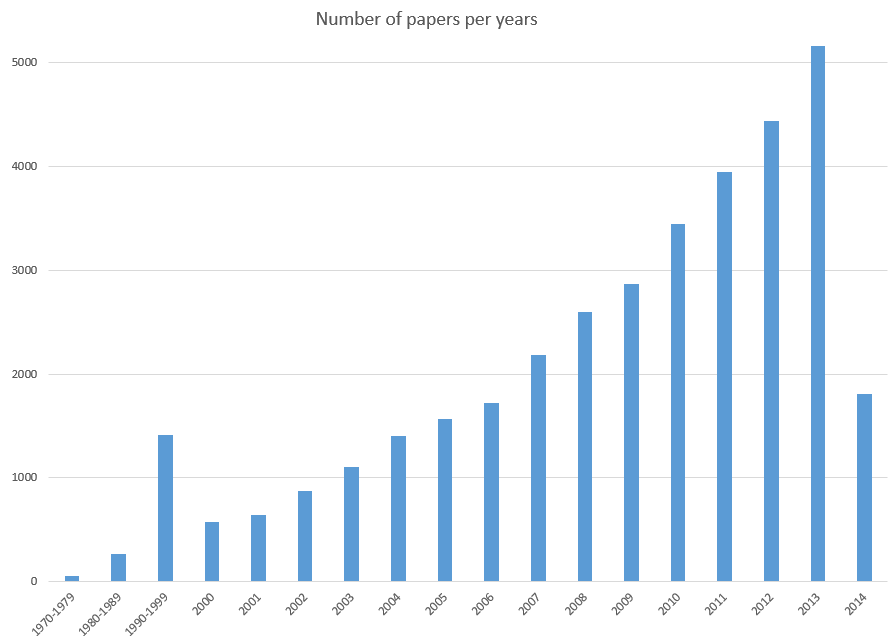
\includegraphics[width=0.98\columnwidth]{Figures/Figure1.png}
\caption{\label{dist1}Distribution of papers per year.}
\end{figure}

If we look at distribution of papers per country of origin of journal where they were publish, then we can conclude that our data set is bias towards journals from the US as they make more than 50 \% of our data set (see Figure \ref{dist2}).

\begin{figure}[h!]
\centering
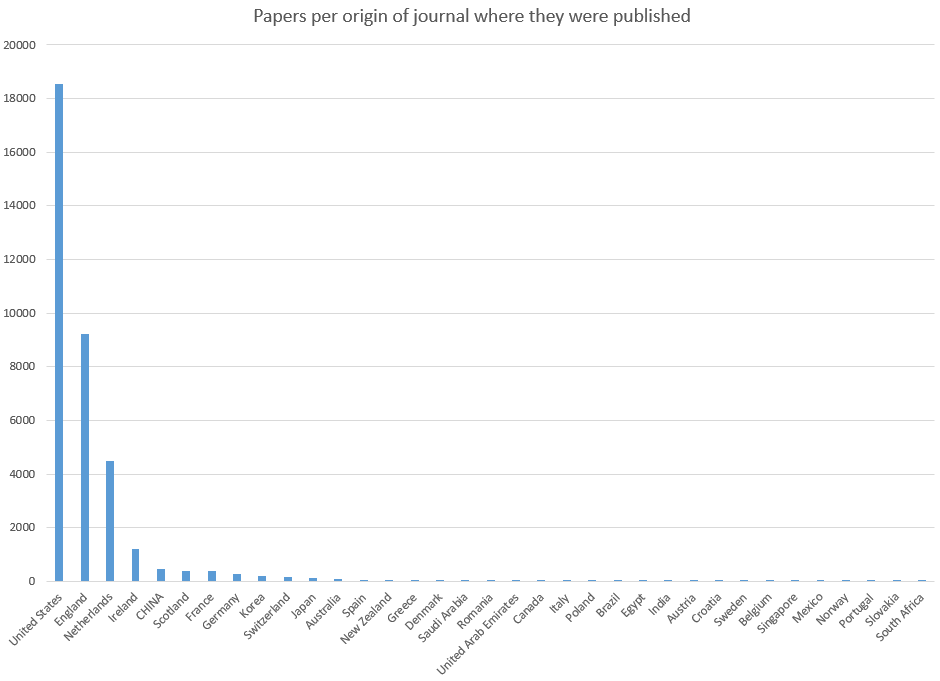
\includegraphics[width=0.98\columnwidth]{Figures/Figure2.png}
\caption{\label{dist2}Distribution of papers per country origin of journal.}
\end{figure}

\section{Initial results}

\bibliographystyle{unsrt}
\bibliography{refs}

\enddocument